\section{Robustheit}\label{sec:robustheit}

Die Robustheit der Modelle wird anhand zweier Kriterien bewertet: der Varianz der F1-Scores über die verschiedenen Seeds und der Anzahl der Retries, die erforderlich waren, um eine formatkorrekte JSON-Antwort von den \acp{LLM} in der Klassifizierungspipeline zu erhalten. Beide Größen geben Aufschluss darüber, wie stabil ein Modell im produktiven Einsatz ist.

Abbildung \ref{fig:results-evaluation-robustness-f1-std} zeigt die Standardabweichungen der F1‑Scores über fünf unabhängige Läufe mit unterschiedlichen Seeds. Die Mehrzahl der Modelle weisen Werte von deutlich unter $0{,}02$ auf. Sie liefern damit weitgehend gleiche Ergebnisse, unabhängig vom gewählten Seed, und gelten als stabil. Dazu zählen \texttt{Gemma-3-12B-it}, \texttt{Mistral-Large-Instruct-2411}, \texttt{GPT-OSS-120B} und \texttt{DeepSeek-R1-Distill-\linebreak~Qwen-14B}.

\begin{figure}[h]
    \centering
    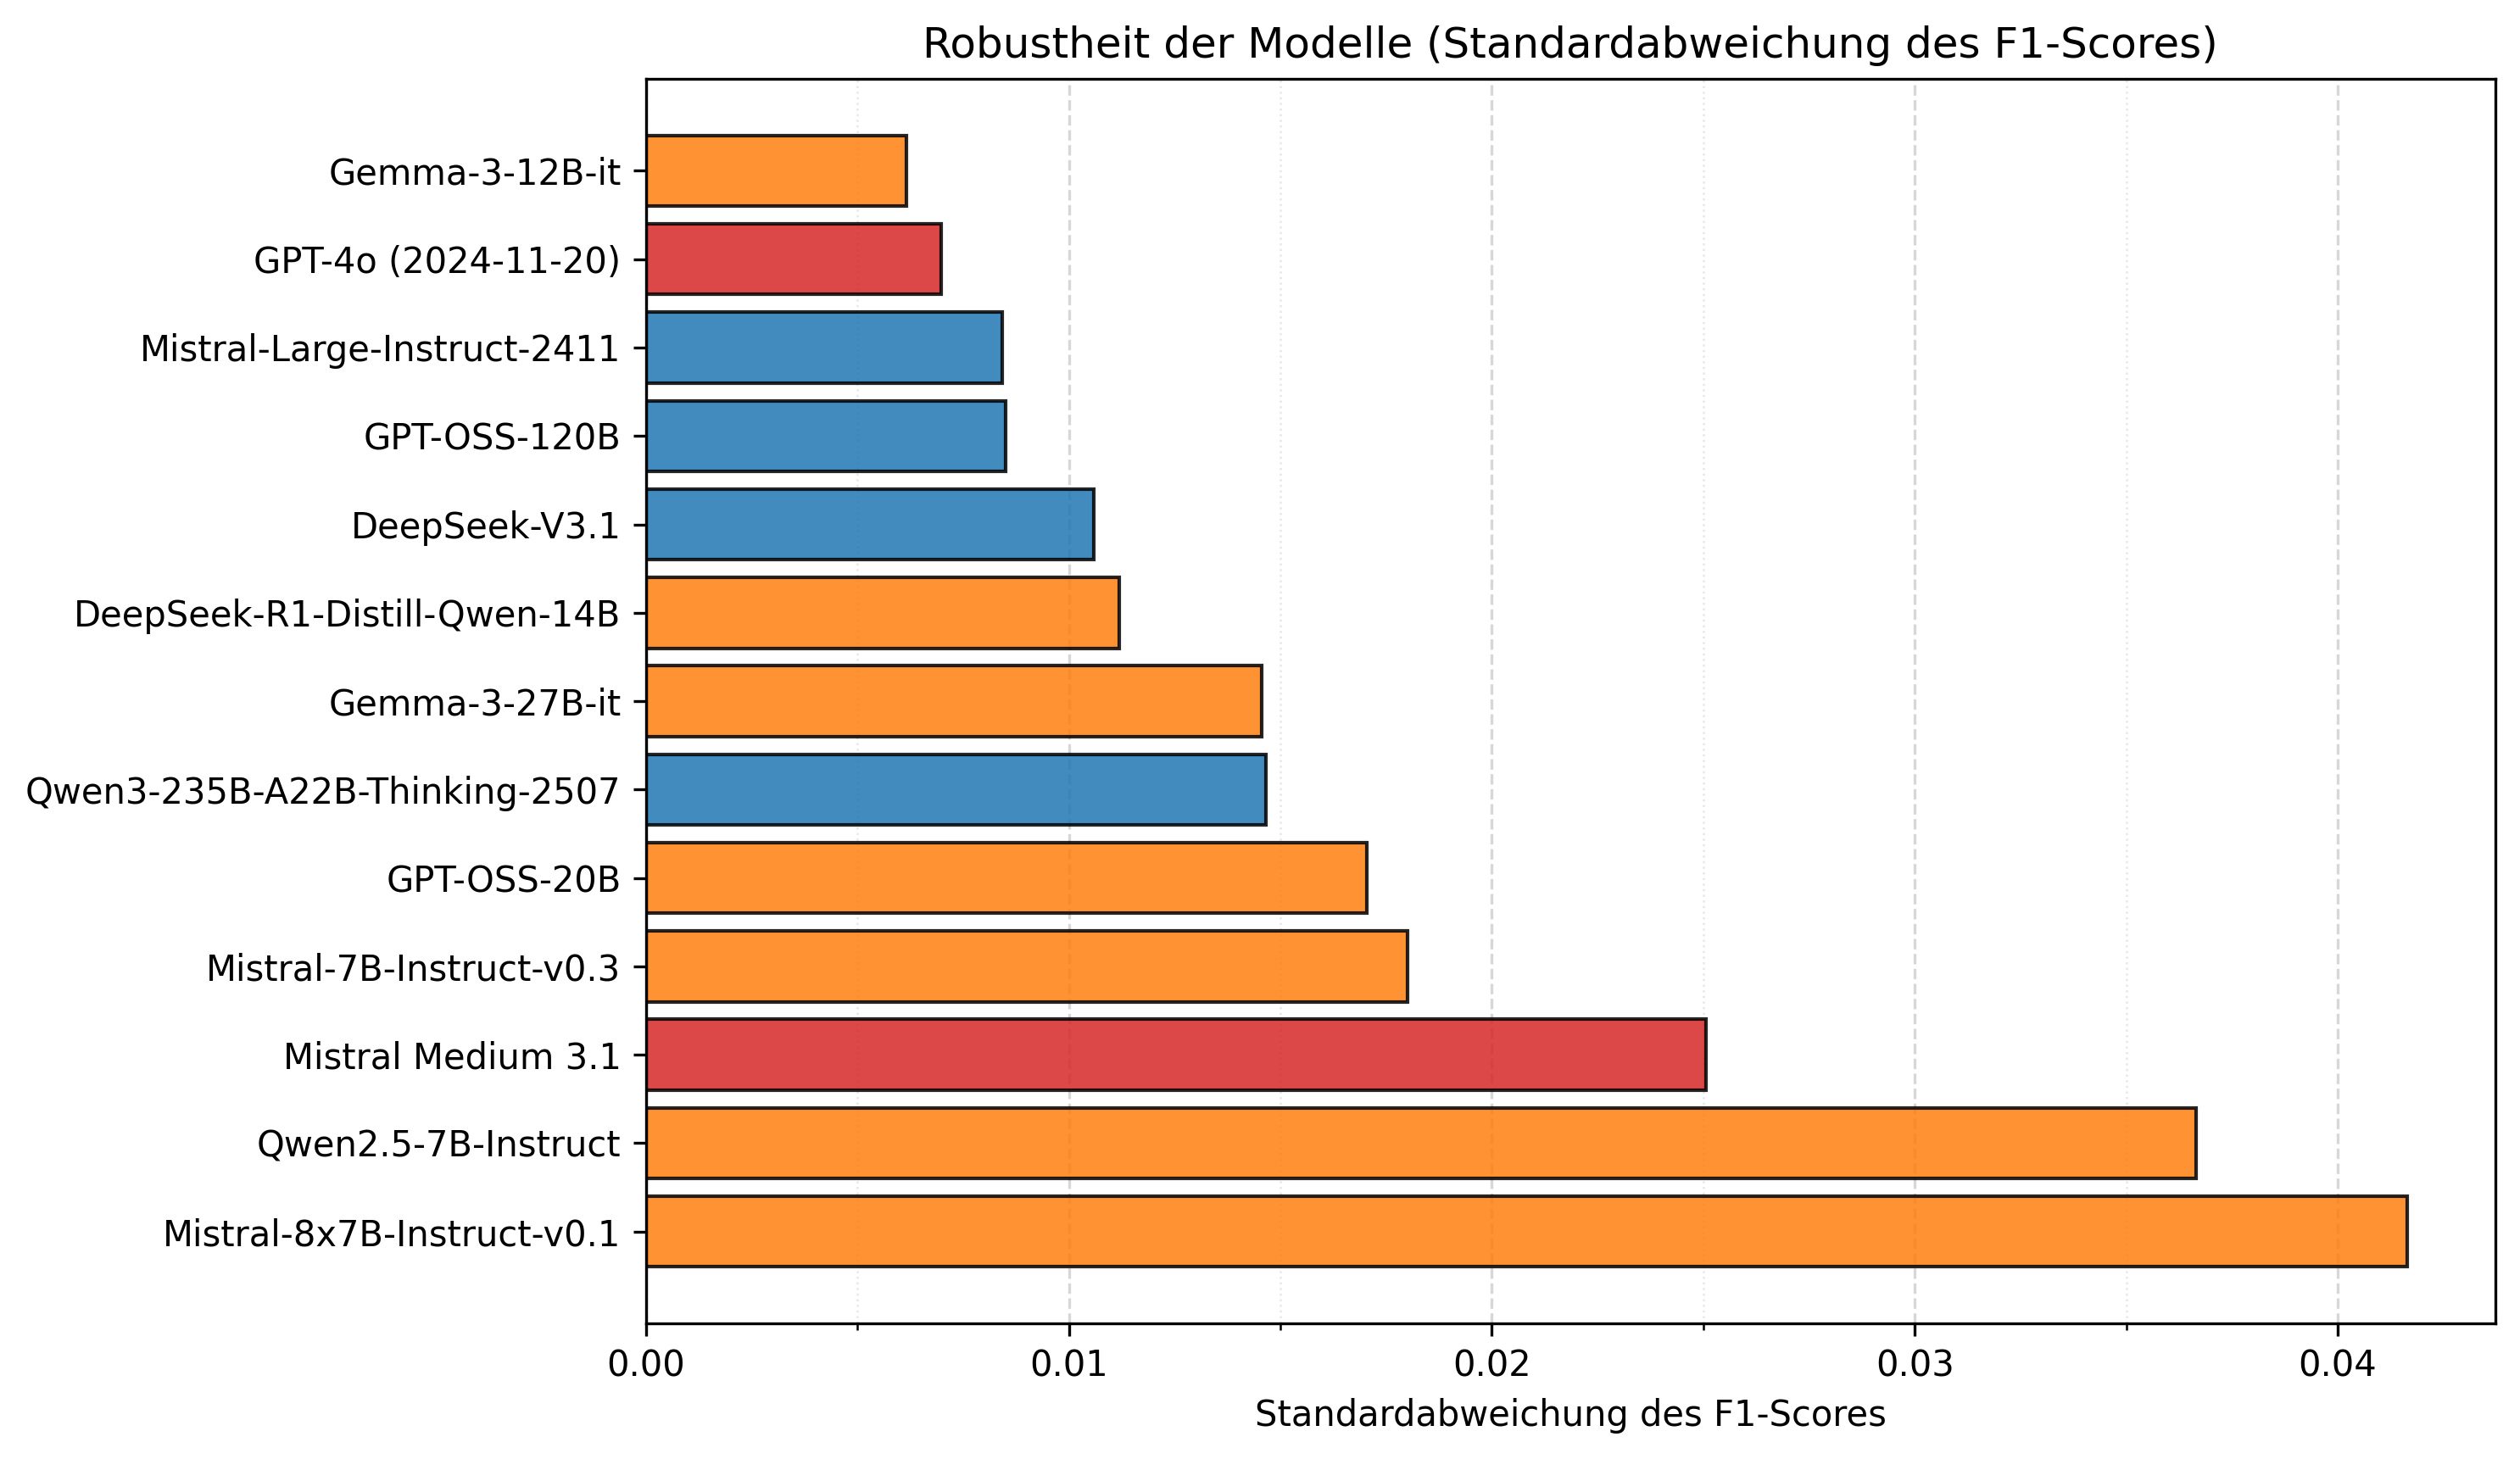
\includegraphics[width=0.88\textwidth]{images/results/evaluation_robustness_f1_std}
    \caption{Robustheit der Modelle gemessen an der Standardabweichung des F1-Scores über alle Wiederholungen hinweg.}
    \label{fig:results-evaluation-robustness-f1-std}
\end{figure}

Demgegenüber weisen \texttt{Mistral Medium 3.1}, \texttt{Qwen2.5-7B-Instruct} und vor allem \texttt{Mixtral-8x7B-Instruct-v0.1} mit Standardabweichungen zwischen $0{,}025$ und über $0{,}04$ eine deutlich höhere Varianz auf. Dies bedeutet, dass ihre Leistung stärker vom gewählten Seed abhängt, was die Vergleichbarkeit und Zuverlässigkeit verringert.

Neben der Varianz des F1-Scores ist auch entscheidend, wie oft das Modell nachgefragt werden muss, bis eine gültige JSON-Struktur zurückgegeben wird. Abbildung \ref{fig:results_evaluation_amount_of_retries} zeigt die durchschnittliche Anzahl notwendiger Retries pro Modell über 25 Testfälle. Die meisten Modelle lieferten bereits im ersten Versuch oder nach maximal einem zusätzlichen Aufruf eine korrekte Antwort. Hervorzuheben sind\linebreak~\texttt{DeepSeek-R1-Distill-Qwen-14B}, \texttt{GPT-4o}, \texttt{Gemma-3-12B-it} und \texttt{Mistral-\linebreak~Large-Instruct-2411}, die keinerlei Retries benötigten.

\begin{figure}[htbp]
    \centering
    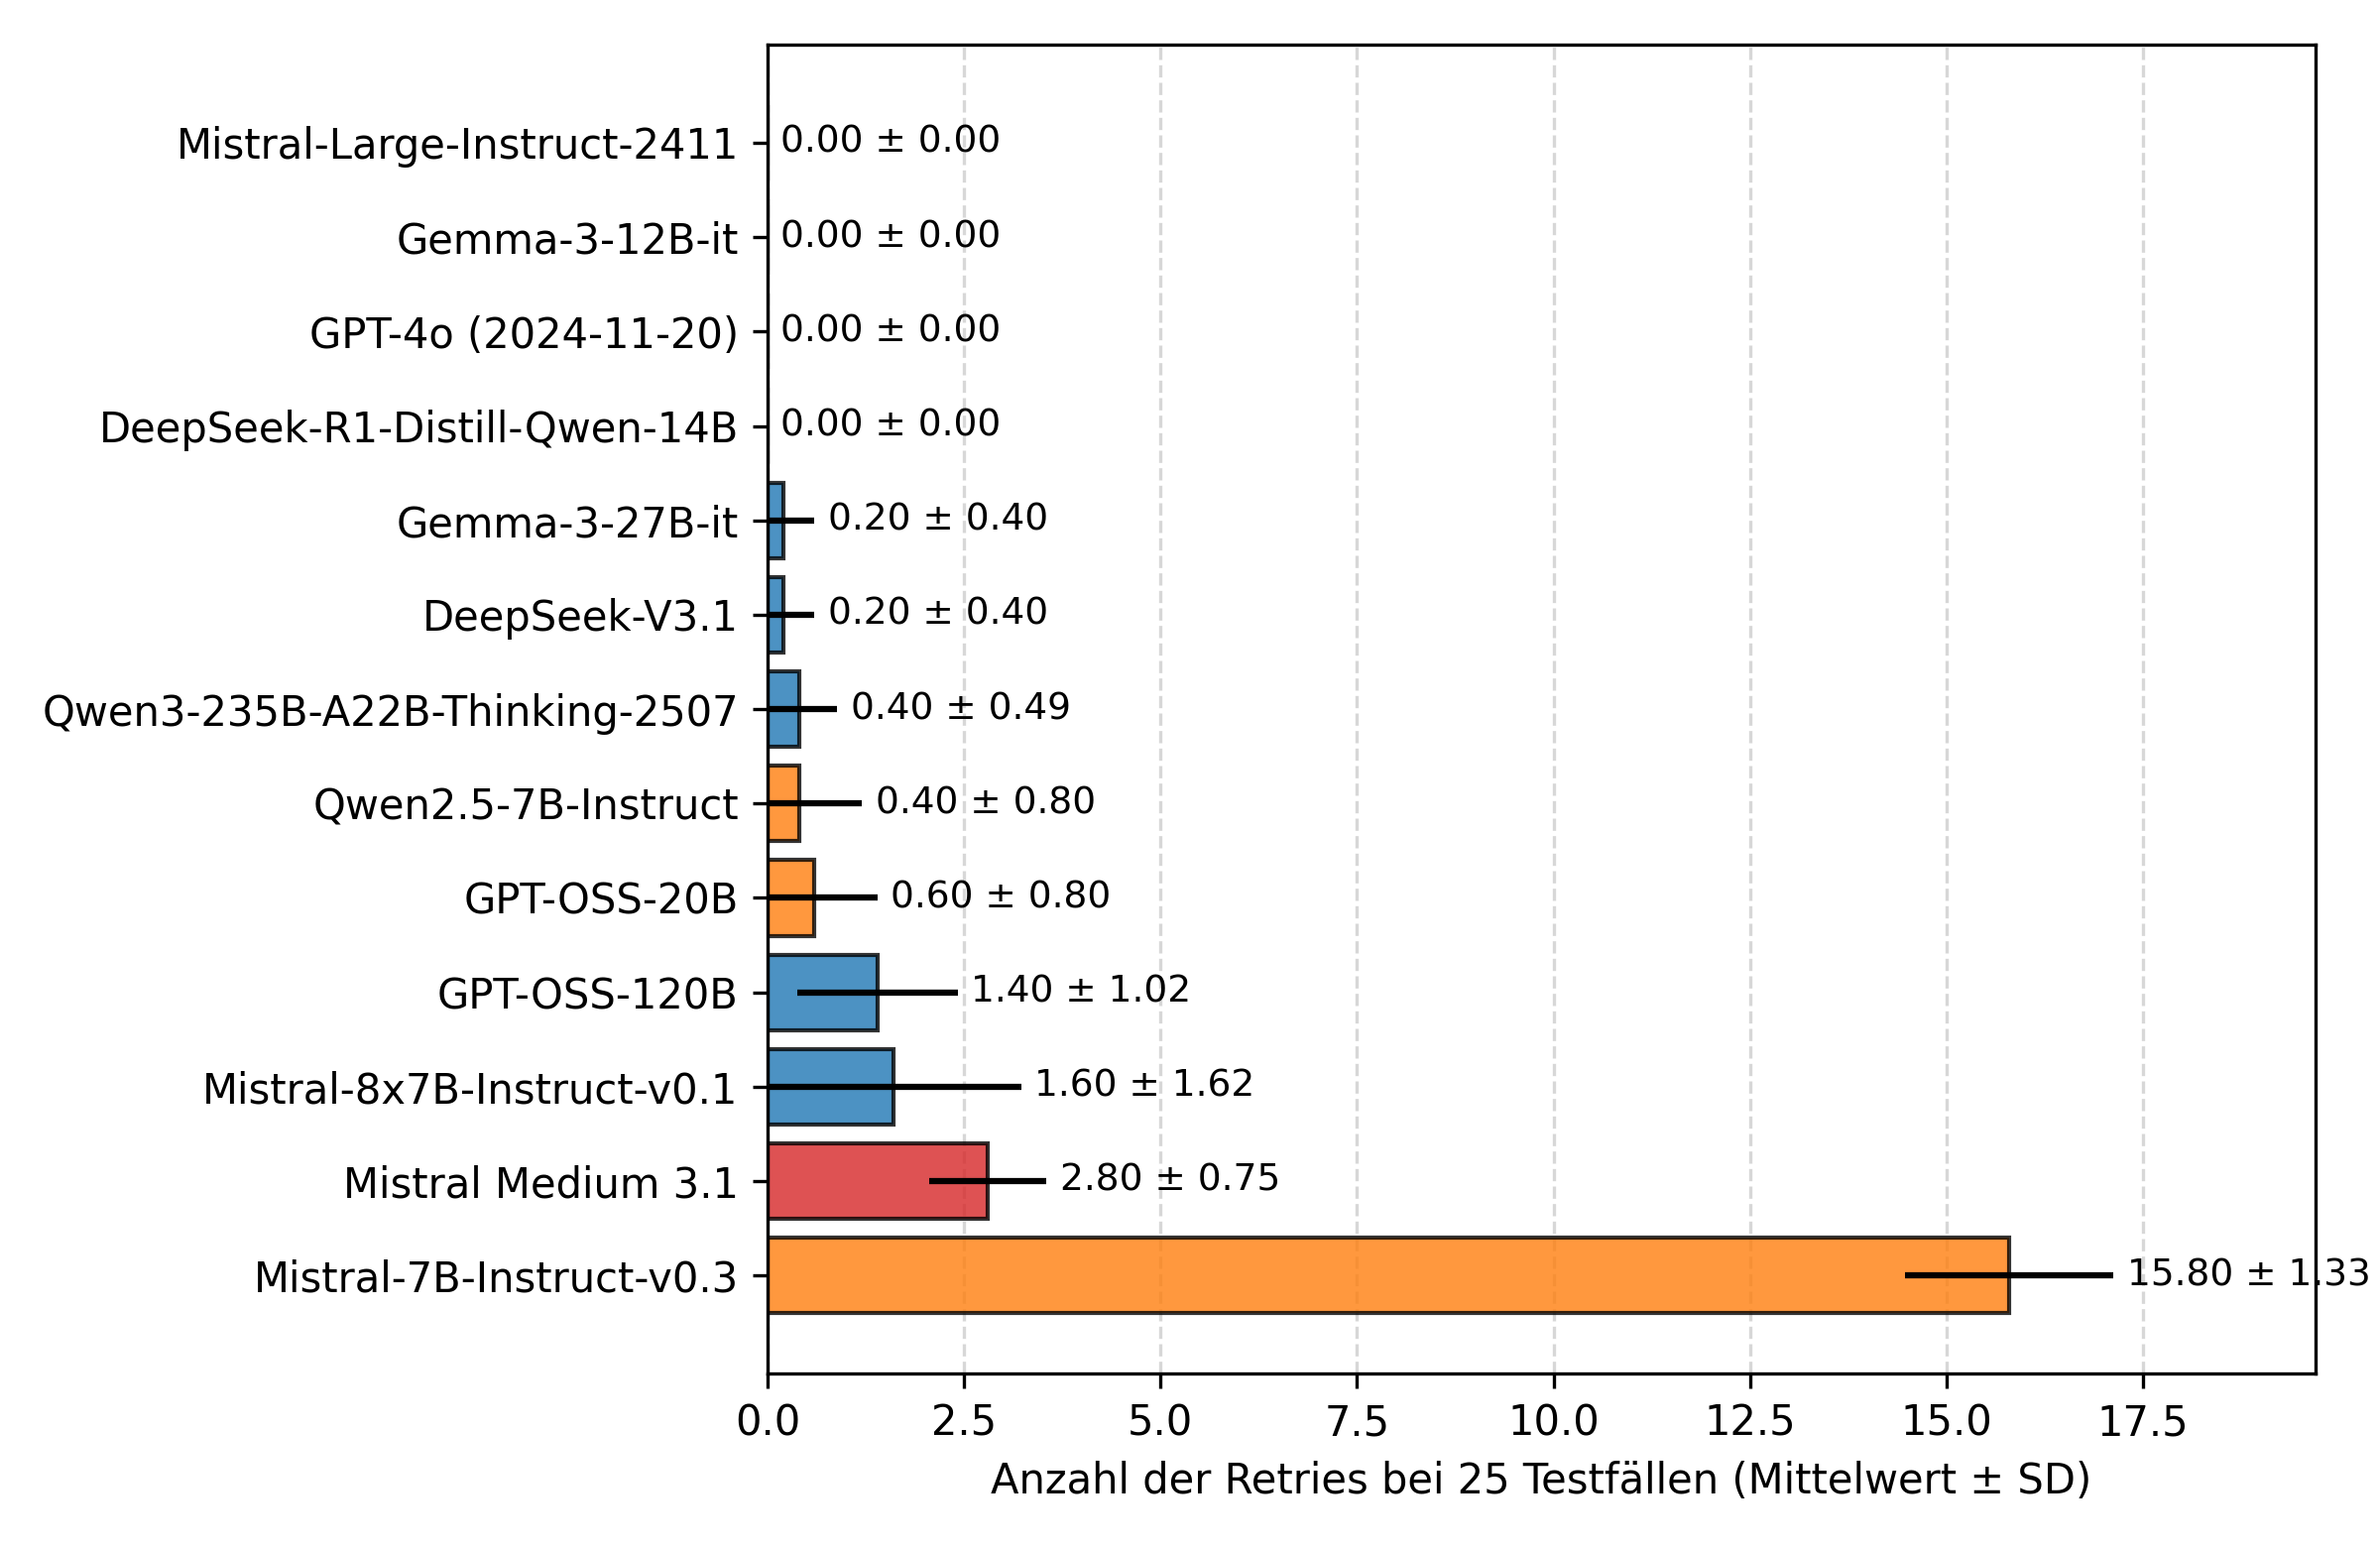
\includegraphics[width=0.95\textwidth]{images/results/evaluation_amount_of_retries_}
    \caption{Durchschnittliche Anzahl der Retries, die notwendig waren, um für alle 25 Testfälle eine formatkorrekte JSON-Antwort zu erhalten.}
    \label{fig:results_evaluation_amount_of_retries}
\end{figure}

Am anderen Ende des Spektrums steht \texttt{Mistral-7B-Instruct-v0.3}, das im Mittel $15{,}8$ zusätzliche Aufrufe benötigte, was im durchschnitt etwa $0{,}63$ Retries pro Testfall entspricht. Diese hohe Zahl verdeutlicht, dass das Modell Schwierigkeiten hat, die vorgegebenen Formatierungsregeln zuverlässig einzuhalten.

In Kombination mit der geringen Varianz sind \texttt{Gemma-3-12B-it}, \texttt{Mistral-Large-\linebreak~Instruct-2411} und \texttt{DeepSeek-R1-Distill-Qwen-14B} die robustesten Modelle: Sie liefern konsistente Ergebnisse und halten das Ausgabeschema zuverlässig ein. Modelle wie \texttt{Mistral Medium 3.1}, \texttt{Qwen2.5-7B-Instruct} und \texttt{Mixtral-8x7B-\linebreak~Instruct-v0.1} sind hingegen anfälliger für Schwankungen und erfordern häufiger Wiederholungen.